\chapter{Farbdarstellungen, Hadronen und Confinement}

\paragraph{Ein kurzes einleitendes Zwischenspiel.}
Bevor wir zur Gruppentheorie zurückkehren, sei ein unverhohlenes Eigenlob erlaubt. \emph{Der Krieg um das Schwarze Loch} erzählt von der langjährigen Auseinandersetzung mit Stephen Hawking darüber, ob Schwarze Löcher Quanteninformation zerstören. Das Buch hält auch eine Grausamkeit fest, die theoretischen Physikern eigentümlich ist: nicht nur Schrödingers Katze, sondern auch Susskinds Fisch und seinen unglücklichen Weg hinunter in die Toilette. Damit wäre diese Pflicht erfüllt; kehren wir zu Alice und Bob zurück. Alice leidet noch immer, denn Bob lässt sie weiterhin Gruppentheorie lernen.

\lectureoverview{Eine Symmetrie wird durch ihre Wirkung auf Zustände physikalisch. Wir beginnen mit Rotationen, um Darstellungen und Erzeugende einzuführen, und wiederholen die Konstruktion anschließend für Farbe \(SU(3)\). Farbdarstellungen setzen sich zu Hadronen zusammen, und ihre Dynamik erklärt, warum isolierte Farbe niemals beobachtet wird.}

\section{Die Gruppe und die Objekte, auf die sie wirkt}

In jeder Diskussion über Symmetrien gibt es zwei Grundgedanken. Erstens eine abstrakte Gruppe: eine Menge von Operationen mit einem Multiplikationsgesetz, einem Einselement und inversen Elementen. Zweitens die Objekte, auf die diese Operationen wirken. Die beiden Gedanken lassen sich unterscheiden, in der Physik aber nicht voneinander trennen. Eine Symmetrie ist relevant, weil sie physikalische Zustände, Felder, Koordinaten oder Observablen transformiert.

\begin{classroomqa}
\audiencequestion{Eine Gruppe wurde sowohl als abstrakte Multiplikationstafel als auch als Matrizen beschrieben, die auf physikalische Objekte wirken. Lassen sich diese beiden Aspekte voneinander trennen?
\lecturetimestamp{00:01:58}}
\lecturerresponse{Es handelt sich um verschiedene Beschreibungsebenen, die jedoch vollständig miteinander verknüpft sind. Eine Rotation existiert als abstrakte Operation, bevor wir festlegen, worauf sie wirkt. Die Physik fragt dann, wie dieselbe Operation auf die für ein bestimmtes System relevanten Zustände und Größen wirkt. Die Matrizen geben diese konkrete Wirkung an und bewahren dabei das abstrakte Multiplikationsgesetz.}
\end{classroomqa}

Räumliche Rotationen sind das anschaulichste Beispiel. Klassisch kann dieselbe Rotation auf die Koordinaten eines Teilchens, auf die Richtung eines Magneten oder auf einen beliebigen anderen Vektor wirken. In der Quantenmechanik liegen Zustände in einem linearen Vektorraum, daher wird eine Rotation durch einen linearen Operator auf diesem Raum dargestellt. Bezeichnet \(g\) ein abstraktes Gruppenelement und \(D(g)\) dessen Matrixdarstellung, so bedeutet Konsistenz
\begin{equation}
D(g_1g_2)=D(g_1)D(g_2),
\qquad
D(e)=\boldsymbol 1.
\end{equation}
Die Matrizen müssen nicht wie die abstrakten Operationen aussehen, aber ihre Multiplikation muss die Gruppenmultiplikation reproduzieren.
\editorialnote{Die Homomorphiegleichung formuliert ausdrücklich die im Text beschriebene Entsprechung zwischen Gruppen- und Matrizenmultiplikation.}

Die Dimension der Matrix wird durch den Zustandsraum bestimmt, nicht allein durch die abstrakte Gruppe. Betrachten wir nur den Spin eines Elektrons, gibt es zwei orthogonale Möglichkeiten: Spin nach oben und Spin nach unten. Ein Zustand ist dann ein Spaltenvektor mit zwei Komponenten. Rotationen wirken daher durch \(2\times2\)-Matrizen. Für zwei Spin-ein-Halb-Objekte gibt es vier Basiszustände,
\begin{equation}
\ket{\uparrow\uparrow},\qquad
\ket{\uparrow\downarrow},\qquad
\ket{\downarrow\uparrow},\qquad
\ket{\downarrow\downarrow},
\end{equation}
und die induzierte Wirkung auf dem kombinierten Raum ist vierdimensional.

Die bekannte Abfolge lautet
\begin{equation}
\begin{array}{c|c|c}
\text{spin} & \text{number of states} & \text{matrix dimension}\\
\hline
0 & 1 & 1\times1\\
\frac12 & 2 & 2\times2\\
1 & 3 & 3\times3\\
\frac32 & 4 & 4\times4
\end{array}
\end{equation}
und so weiter. Ein Spin-null-Zustand bildet die triviale Darstellung: Jede Rotation lässt ihn unverändert. Die einzeilige Matrix ist einfach \(1\). Ein Spin-eins-Zustand hat drei Komponenten, und seine Rotationsmatrizen sind die vertrauten dreidimensionalen Vektorrotationen. Allgemeiner hat Spin \(j\) genau \(2j+1\) Zustände.

Die Darstellung kann auch unendlichdimensional sein. Beschreiben wir die gesamte Bahnbewegung eines Elektrons statt nur seines Spins, enthält ein Zustand eine Amplitude für jede Position oder, gleichwertig, für jeden Impuls. Der Rotationsoperator wirkt dann auf einem unendlichdimensionalen Raum von Wellenfunktionen. Dieselbe abstrakte Rotationsgruppe besitzt also triviale, zweidimensionale, dreidimensionale und unendlichdimensionale Darstellungen. Diese Tatsache werden wir wiederverwenden, wenn wir von Spin zu Farbe übergehen.

\section{Warum Spinrotationen speziell unitär sind}

Betrachten wir wieder den Spin eines einzelnen Elektrons und lassen seine Bahnbewegung außer Acht. Eine Rotation wird durch eine unitäre \(2\times2\)-Matrix \(U\) dargestellt,
\begin{equation}
U^\dagger U=\boldsymbol 1,
\qquad
U^{-1}=U^\dagger.
\label{eq:l4-unitarity}
\end{equation}
Die inverse Transformation muss die Rotation rückgängig machen, und Unitarität erhält die Norm und damit jede Wahrscheinlichkeit.

Eine allgemeine \(2\times2\)-Matrix mit komplexen Einträgen enthält vier komplexe beziehungsweise acht reelle Parameter. Gleichung~\eqref{eq:l4-unitarity} legt vier unabhängige reelle Bedingungen fest, sodass vier Parameter übrig bleiben. Eine gewöhnliche räumliche Rotation hat nur drei: Zwei Parameter bestimmen die Achse, einer den Winkel. Die unitäre Matrix enthält also eine Phase zu viel. Die zusätzliche Bedingung lautet
\begin{equation}
\det U=1.
\label{eq:l4-det-one}
\end{equation}
Die Parameterzahl ist dann
\begin{equation}
8-4-1=3.
\end{equation}

Die Bedingung, dass die Determinante eins ist, bleibt bei Multiplikation erhalten, denn
\begin{equation}
\det(AB)=\det A\,\det B.
\end{equation}
Haben zwei Matrizen jeweils Determinante eins, so gilt das auch für ihr Produkt. Die Bedingung ist außerdem mit der Unitarität vereinbar. Bilden wir die Determinante von Gleichung~\eqref{eq:l4-unitarity}, so folgt
\begin{equation}
1=\det(U^\dagger U)
=\det(U^\dagger)\det U
=(\det U)^*\det U.
\end{equation}
Die Determinante einer unitären Matrix liegt folglich auf dem Einheitskreis:
\begin{equation}
\det U=e^{i\phi}.
\end{equation}

\begin{classroomqa}
\audiencequestion{Muss die Determinante aufgrund der Unitarität reell sein?
\lecturetimestamp{00:12:10}}
\lecturerresponse{Nein. Die Unitarität verlangt lediglich, dass ihr Betrag eins ist. Die Determinante kann eine beliebige reine Phase \(e^{i\phi}\) sein. Bei einer zweidimensionalen Matrix entfernt die Multiplikation von \(U\) mit \(e^{-i\phi/2}\) diese gemeinsame Phase und ergibt eine Matrix mit Determinante eins.}
\end{classroomqa}

Tatsächlich gilt: Wenn
\begin{equation}
V=e^{-i\phi/2}U,
\end{equation}
dann ist \(V\) weiterhin unitär und
\begin{equation}
\det V=e^{-i\phi}\det U=1.
\end{equation}
Die unitären Matrizen mit Determinante eins bilden \(SU(2)\).

Dabei gibt es eine Feinheit. Es liegt nahe zu sagen, \(SU(2)\) sei einfach die Gruppe der Rotationen im dreidimensionalen Raum, doch die Zuordnung ist zweifach. Die Matrizen \(U\) und \(-U\) wirken unterschiedlich auf einen Spinor, entsprechen aber derselben Rotation eines gewöhnlichen Vektors. Daher gilt
\begin{equation}
SU(2)/\{\boldsymbol 1,-\boldsymbol 1\}\simeq SO(3).
\end{equation}
Für die vorliegende Diskussion sind die lokale Multiplikationsstruktur und die drei Erzeugenden entscheidend. Die zweifache Überlagerung erklärt jedoch die Zweideutigkeit von Spin-ein-Halb-Rotationen.

\section{Infinitesimale Transformationen und ihre Erzeugenden}

Eine endliche Rotation lässt sich aus vielen sehr kleinen Rotationen aufbauen. Ein Gruppenelement nahe dem Einselement heißt infinitesimal. Kennt man alle infinitesimalen Richtungen, lassen sich in einer zusammenhängenden Gruppe durch wiederholte Multiplikation endliche Transformationen rekonstruieren. Für die Physik ist noch wichtiger, dass die Operatoren, welche diese infinitesimalen Transformationen erzeugen, die der Symmetrie zugeordneten Erhaltungsgrößen sind.

Schreiben wir ein Element nahe dem Einselement als
\begin{equation}
U=\boldsymbol 1+i\epsilon T,
\qquad |\epsilon|\ll1.
\label{eq:l4-infinitesimal-u}
\end{equation}
Der Faktor \(i\) ist eine zweckmäßige Konvention. Setzen wir dies in die Unitaritätsbedingung ein und verwerfen Terme der Ordnung \(\epsilon^2\), so erhalten wir
\begin{align}
(\boldsymbol 1+i\epsilon T)
(\boldsymbol 1-i\epsilon T^\dagger)&=\boldsymbol 1,
\\
i\epsilon(T-T^\dagger)&=0,
\\
T&=T^\dagger.
\label{eq:l4-hermitian-generator}
\end{align}
Der Erzeugende ist hermitesch, wie es eine quantenmechanische Observable sein muss.

\begin{figure}[htbp]\centering
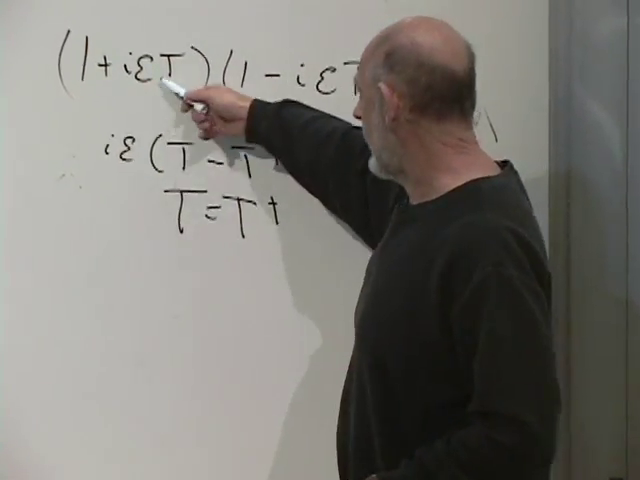
\includegraphics[width=0.62\textwidth]{lecture_04_figure_03.png}\caption{Die Unitaritätsrechnung nahe dem Einselement endet mit \(T=T^\dagger\).}\lectureframe{00:23:28}\end{figure}

Drei linear unabhängige Erzeugende entsprechen räumlichen Rotationen, denn es gibt drei unabhängige infinitesimale Achsen. Eine kleine Rotation um eine beliebige Richtung lässt sich aus kleinen Rotationen um \(x\), \(y\) und \(z\) zusammensetzen. Die entsprechenden Erzeugenden sind die Drehimpulsoperatoren \(J_x,J_y,J_z\). Ihre Kommutatoren kodieren die Nichtvertauschbarkeit von Rotationen:
\begin{equation}
[J_i,J_j]=i\epsilon_{ijk}J_k.
\label{eq:l4-angular-momentum-algebra}
\end{equation}
Durch wiederholte infinitesimale Rotationen entsteht dann eine endliche Rotation.

Wir haben die Unitarität verwendet, aber noch nicht die Bedingung, dass die Determinante eins ist. Für eine beliebige kleine Matrix \(m\) gilt
\begin{equation}
\det(\boldsymbol 1+\epsilon m)
=1+\epsilon\,\operatorname{tr}m+O(\epsilon^2).
\label{eq:l4-det-expansion}
\end{equation}

\begin{figure}[htbp]\centering
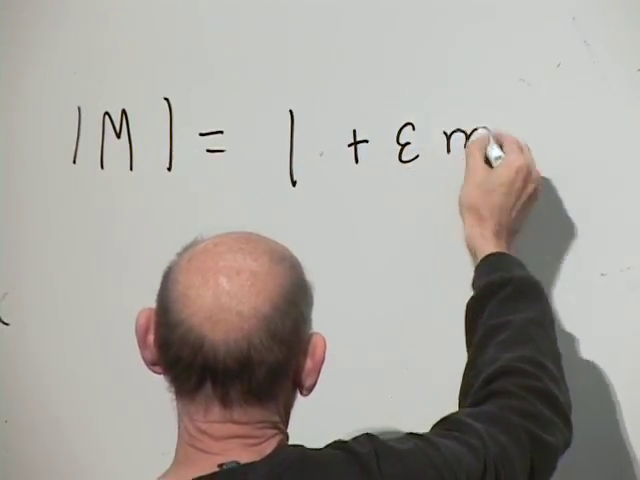
\includegraphics[width=0.62\textwidth]{lecture_04_figure_02.png}\caption{Die Entwicklung der Determinante in erster Ordnung, wie sie an der Tafel beginnt.}\lectureframe{00:21:51}\end{figure}

Wenden wir Gleichung~\eqref{eq:l4-det-expansion} auf Gleichung~\eqref{eq:l4-infinitesimal-u} an, so erhalten wir
\begin{equation}
\det U
=1+i\epsilon\,\operatorname{tr}T+O(\epsilon^2).
\end{equation}
Die Bedingung der speziellen Unitarität verlangt daher
\begin{equation}
\operatorname{tr}T=0.
\label{eq:l4-traceless-generator}
\end{equation}
Die Erzeugenden von \(SU(2)\) sind genau die spurfreien hermiteschen \(2\times2\)-Matrizen. Dieser Vektorraum hat Dimension drei. Eine Standardbasis bilden die Pauli-Matrizen:
\begin{equation}
\begin{aligned}
\sigma_x&=
\begin{pmatrix}0&1\\1&0\end{pmatrix},
&
\sigma_y&=
\begin{pmatrix}0&-i\\i&0\end{pmatrix},
\\[0.4em]
\sigma_z&=
\begin{pmatrix}1&0\\0&-1\end{pmatrix}.
\end{aligned}
\end{equation}
Für eine Spin-ein-Halb-Darstellung kann man \(J_i=\sigma_i/2\) wählen. Eine endliche Rotation um den Winkel \(\theta\) um die Richtung \(\hat{\boldsymbol n}\) lautet dann
\begin{equation}
U(\hat{\boldsymbol n},\theta)
=\exp\!\left(-i\theta\,
\hat{\boldsymbol n}\cdot\boldsymbol\sigma/2\right).
\end{equation}
\editorialnote{Die endliche Exponentialdarstellung vervollständigt die übliche Behandlung der infinitesimalen Erzeugenden. Die Quelle betont wiederholte kleine Rotationen, statt diese Formel ausdrücklich anzugeben.}

\begin{classroomqa}
\audiencequestion{Gibt es also drei unabhängige spurfreie hermitesche \(2\times2\)-Matrizen?
\lecturetimestamp{00:24:07}}
\lecturerresponse{Ja. Es sind die drei Pauli-Matrizen. Für spezielle unitäre \(3\times3\)-Matrizen beträgt die entsprechende Anzahl acht; eine konventionelle Basis bilden die acht Gell-Mann-Matrizen.}
\end{classroomqa}

\begin{classroomqa}
\audiencequestion{Ist diese ``Acht'' dieselbe wie beim Achtfachen Weg und bei den acht Gluonen?
\lecturetimestamp{00:24:43}}
\lecturerresponse{Die Mathematik beruht auf derselben Art von Darstellungstheorie \(SU(3)\), aber man muss angeben, welche Symmetrie \(SU(3)\) wirkt. Die historische Flavor-Symmetrie des Achtfachen Weges ist nicht die Farbsymmetrie \(SU(3)\). Die acht Gluonen gehören zur adjungierten Darstellung der Farbsymmetrie \(SU(3)\).}
\end{classroomqa}

\section{Von SU(2) zu Farb-SU(3)}

Vergrößern wir nun die Matrizen von \(2\times2\) auf \(3\times3\). Eine allgemeine komplexe \(3\times3\)-Matrix hat neun komplexe Einträge, also achtzehn reelle Parameter. Die Bedingung \(U^\dagger U=\boldsymbol 1\) liefert neun reelle Bedingungen, und \(\det U=1\) fügt eine weitere hinzu. Somit gilt
\begin{equation}
18-9-1=8.
\end{equation}
Es gibt acht unabhängige infinitesimale Richtungen und acht spurfreie hermitesche Erzeugende. Anders als \(SU(2)\) ist diese Gruppe nicht die Rotationsgruppe des gewöhnlichen dreidimensionalen Raums. Sie ist eine innere Symmetrie, die auf Farbe wirkt.

Bevor wir diese Darstellungen Quarks zuordnen, erinnern wir uns daran, wie zusammengesetzte Darstellungen entstehen. Legt man zwei Spin-ein-Halb-Systeme übereinander und lässt ihre Bahnbewegung außer Acht, erhält man vier Produktzustände. Eine Rotation mischt jedoch nicht alle vier unzerlegbar miteinander. Drei Kombinationen transformieren wie Spin eins:
\begin{align}
\ket{1,1}&=\ket{\uparrow\uparrow},\\
\ket{1,0}&=\frac{1}{\sqrt2}
(\ket{\uparrow\downarrow}+\ket{\downarrow\uparrow}),\\
\ket{1,-1}&=\ket{\downarrow\downarrow},
\end{align}
während die vierte wie Spin null transformiert:
\begin{equation}
\ket{0,0}=\frac{1}{\sqrt2}
(\ket{\uparrow\downarrow}-\ket{\downarrow\uparrow}).
\end{equation}
Damit gilt
\begin{equation}
\boldsymbol 2\otimes\boldsymbol 2
=\boldsymbol 3\oplus\boldsymbol 1.
\label{eq:l4-two-spin-decomposition}
\end{equation}
Die ausgerichteten Zustände bilden die Zustände mit \(m=\pm1\), der symmetrische Zustand mit Projektion null vervollständigt das Triplett, und die antisymmetrische Kombination ist das Singulett. Darin liegt die allgemeine Logik der Addition von Drehimpulsen und der Kombination von Farbdarstellungen.

Dieselbe Singulett--Triplett-Unterscheidung tritt immer auf, wenn zwei Spin-ein-Halb-Freiheitsgrade gekoppelt werden. Im atomaren Wasserstoff bilden Elektron- und Protonenspin Hyperfein-Singulett- und -Triplettzustände. Ortho- und Parawasserstoff verwenden dieselbe Darstellungstheorie für die Kernspins der beiden Protonen in einem \(H_2\)-Molekül.
\editorialnote{Die Quelle verwendet ``Ortho- und Parawasserstoff'' und bezieht sich dabei auf Proton--Elektron-Spins im Wasserstoffatom. Die mathematische Zerlegung ist korrekt; zur Präzisierung werden hier die Bezeichnungen für Molekül und Atom unterschieden.}

\subsection{Das Triplett und das Antitriplett}

Ein einzelnes Quark hat drei Farb-Amplituden. In einer gewählten Basis schreiben wir
\begin{equation}
q=
\begin{pmatrix}
q_r\\q_g\\q_b
\end{pmatrix},
\qquad
q'=Uq,
\qquad U\in SU(3).
\label{eq:l4-quark-triplet}
\end{equation}
Die drei Einträge können Zustandsamplituden eines einzelnen Quarks oder drei Feldoperatoren sein, die rote, grüne und blaue Quarks erzeugen. Die Gruppe mischt die drei Komponenten. Ein Zustand, der zunächst rot ist, wird nach einer Farbtransformation im Allgemeinen zu einer Überlagerung aus Rot, Grün und Blau. Diese fundamentale dreidimensionale Darstellung heißt \(\boldsymbol 3\).

Bei einem Antiquark wirkt die Gruppe durch die komplex konjugierte Darstellung der Quarkdarstellung. Die komplexe Konjugation von Gleichung~\eqref{eq:l4-quark-triplet} ergibt
\begin{equation}
\bar q'=U^*\bar q.
\end{equation}
Diese Darstellung wird mit \(\bar{\boldsymbol 3}\) bezeichnet. Die Analogie zu \(U(1)\) liegt auf der Hand: Nimmt ein Elektronenfeld den Faktor \(e^{i\theta}\) auf, so nimmt ein Positronenfeld \(e^{-i\theta}\) auf. Die Farbtransformationen von Quarks und Antiquarks bilden die nichtabelsche Variante dieser konjugierten Zuordnung.

Nahe dem Einselement gilt, wenn
\begin{equation}
U=\boldsymbol 1+i\epsilon T,
\end{equation}
dann
\begin{equation}
U^*=\boldsymbol 1-i\epsilon T^*.
\end{equation}
Die Erzeugenden des Antitripletts sind somit \(-T^*\), also die komplex konjugierten Erzeugenden mit umgekehrtem Vorzeichen. Genau in diesem Sinn tragen Antiquarks entgegengesetzte Farbladungen.

\begin{classroomqa}
\audiencequestion{Was geschieht mit der komplex konjugierten Darstellung im Fall \(SU(2)\)?
\lecturetimestamp{00:36:19}}
\lecturerresponse{Das \(SU(2)\)-Dublett ist ein Sonderfall: Seine komplex konjugierte Darstellung ist nach einer festen Basisänderung mit dem ursprünglichen Dublett äquivalent; diese verwendet den antisymmetrischen Epsilon-Tensor. Für \(SU(3)\) sind \(\boldsymbol 3\) und \(\bar{\boldsymbol 3}\) tatsächlich nicht äquivalente Darstellungen.}
\end{classroomqa}
\editorialnote{Der mathematisch präzise Begriff für die fundamentale Darstellung von \(SU(2)\) lautet pseudoreell, nicht reell. Die Antwort bewahrt die beabsichtigte Unterscheidung der Quelle und korrigiert zugleich die Terminologie.}

\section{Farbdarstellungen kombinieren}

Das Symbol \(\otimes\) bedeutet keine gewöhnliche Multiplikation der danebenstehenden Zahlen. Es bezeichnet die Kombination zweier Zustandsräume. Der entstehende Tensorproduktraum wird anschließend in Teilräume zerlegt, die unter der Gruppenwirkung nicht miteinander vermischt werden.

\subsection{\texorpdfstring{\(\boldsymbol 3\otimes\boldsymbol 3\)}{Zwei Quarks: 33 x }}

Zwei Quarks haben neun Farb-Basiszustände: Rot--Rot, Rot--Grün, Rot--Blau sowie die sechs übrigen geordneten Paare. Ordnen wir die beiden Farb-Indizes in einen symmetrischen und einen antisymmetrischen Anteil. Der symmetrische Anteil hat sechs unabhängige Komponenten, der antisymmetrische drei. Unter \(SU(3)\) gilt
\begin{equation}
\boldsymbol 3\otimes\boldsymbol 3
=\boldsymbol 6\oplus\bar{\boldsymbol 3}.
\label{eq:l4-three-times-three}
\end{equation}

\begin{figure}[htbp]\centering
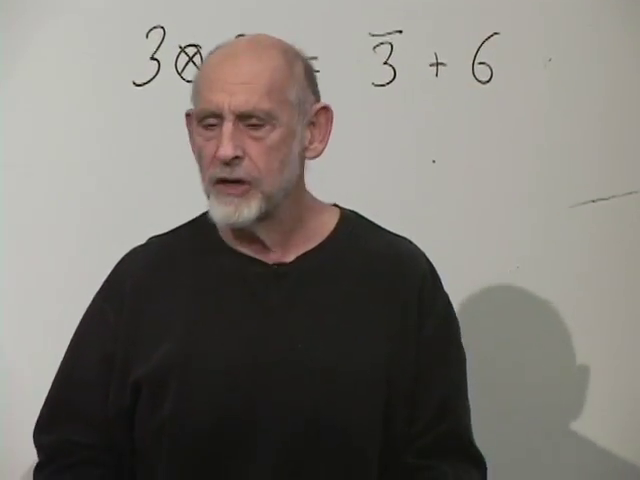
\includegraphics[width=0.68\textwidth]{lecture_04_figure_04.png}\caption{Das Produkt zweier Quarks zerfällt in ein Antitriplett und ein Sextett.}\lectureframe{00:39:33}\end{figure}

Das Antitriplett lässt sich ausdrücklich darstellen, indem man zwei Quark-Indizes mit dem invarianten Epsilon-Tensor kontrahiert:
\begin{equation}
(qq)^k_{\bar 3}
=\frac{1}{\sqrt2}\epsilon^{kij}q_iq_j.
\end{equation}
Dieses Objekt hat drei Komponenten und transformiert wie ein Antiquark. Die sechs symmetrischen Kombinationen bilden das Sextett. Die Aussage lautet nicht, dass sich zwei Quarks dynamisch in ein Antiquark verwandeln; vielmehr hat ein Sektor ihrer Farb-Wellenfunktion dasselbe Transformationsgesetz wie ein Antiquark.

\subsection{\texorpdfstring{\(\boldsymbol 3\otimes\bar{\boldsymbol 3}\)}{Ein Quark und ein Antiquark: 3 x Anti-3}}

Ein Quark--Antiquark-Farbzustand lässt sich als \(3\times3\)-Matrix \(M_i{}^j=q_i\bar q^j\) auffassen. Jede solche Matrix zerfällt eindeutig in ihre Spur und einen spurfreien Anteil:
\begin{equation}
M=\frac{\operatorname{tr}M}{3}\boldsymbol 1
+\left(M-\frac{\operatorname{tr}M}{3}\boldsymbol 1\right).
\end{equation}
Die Spur ist eine einzelne invariante Komponente, der spurfreie Anteil hat acht Komponenten. Daher gilt
\begin{equation}
\boldsymbol 3\otimes\bar{\boldsymbol 3}
=\boldsymbol 1\oplus\boldsymbol 8.
\label{eq:l4-three-times-threebar}
\end{equation}
Bis auf die Normierung lautet das Singulett
\begin{equation}
\ket{1}_{q\bar q}
=\frac{1}{\sqrt3}
(\ket{r\bar r}+\ket{g\bar g}+\ket{b\bar b}).
\end{equation}
Es kann in nichts anderes transformieren, weil es invariant ist. Die übrigen acht Linearkombinationen mischen sich untereinander. Sie bilden die adjungierte Darstellung, in der auch die acht Erzeugenden transformieren.

\subsection{Drei Quarks}

Kombinieren wir ein drittes Quark mit Gleichung~\eqref{eq:l4-three-times-three}. Der Antitriplett-Zweig ergibt
\begin{equation}
\bar{\boldsymbol 3}\otimes\boldsymbol 3
=\boldsymbol 1\oplus\boldsymbol 8,
\end{equation}
sodass das Produkt aus drei Quarks ein Singulett enthält. Vollständig lautet die Zerlegung
\begin{equation}
\boldsymbol 3\otimes\boldsymbol 3\otimes\boldsymbol 3
=\boldsymbol 1\oplus\boldsymbol 8\oplus\boldsymbol 8
\oplus\boldsymbol{10}.
\label{eq:l4-three-quark-full}
\end{equation}
Das Farbsingulett ist die vollständig antisymmetrische Kombination Rot--Grün--Blau:
\begin{equation}
\ket{1}_{qqq}
=\frac{1}{\sqrt6}\epsilon^{ijk}\ket{q_iq_jq_k}.
\label{eq:l4-baryon-singlet}
\end{equation}
Da \(\epsilon^{ijk}\) verschwindet, wenn zwei Indizes übereinstimmen, enthält jeder von null verschiedene Term genau ein rotes, ein grünes und ein blaues Quark; beim Vertauschen wechseln die Vorzeichen.

\begin{classroomqa}
\audiencequestion{Sind die Kombinationen, die keine Singuletts sind, lediglich unwahrscheinlich, sodass man ihre Wahrscheinlichkeiten vernachlässigen kann?
\lecturetimestamp{00:46:02}}
\lecturerresponse{Nein. Entscheidend ist die Energie, nicht eine geringe Wahrscheinlichkeit. Ein isolierter Zustand, der kein Singulett ist, hätte ein Farbfeld, das bis in beliebig große Entfernung reicht, und würde im Confinement-Bereich unbegrenzte Energie erfordern. Die Dynamik dahinter behandeln wir weiter unten.}
\end{classroomqa}

\subsection{Das Gluonen-Oktett}

Das Gluonenfeld transformiert wie das Oktett in Gleichung~\eqref{eq:l4-three-times-threebar}. Bezüglich der Farbe trägt es einen Triplett- und einen Antitriplett-Index, wobei die Singulett-Spur entfernt ist. Schematisch gilt
\begin{equation}
q\sim\boldsymbol 3,
\qquad
\bar q\sim\bar{\boldsymbol 3},
\qquad
G\sim\boldsymbol 8.
\end{equation}
Diese Symbole bezeichnen Transformationsgesetze; Teilchen sind nicht wörtlich gleich den Zahlen drei und acht.

Die neunte Farb-Kombination aus Quark-- und Antiquark, proportional zur Einheitsmatrix, ist ein Singulett und mischt sich nicht mit dem Oktett. Sie wegzulassen ist daher mathematisch konsistent: Ein \(SU(3)\)-Eichfeld ist spurfrei und hat acht Komponenten, statt der neun eines \(U(3)\)-Eichfelds.

\begin{classroomqa}
\audiencequestion{Warum lässt die Natur das zusätzliche Singulett-Gluon weg?
\lecturetimestamp{00:49:00}}
\lecturerresponse{Die unmittelbare gruppentheoretische Antwort lautet, dass das Singulett ein eigener invarianter Sektor ist. Daher ist das Oktett auch ohne ihn abgeschlossen. Der tieferliegende Grund für die Wahl von \(SU(3)\) statt \(U(3)\) wird hier nicht hergeleitet; er gehört zur Eichstruktur, die aus der Phänomenologie der QCD erschlossen wird.}
\end{classroomqa}

\section{Farbsinguletts als Hadronen}

Die freien Teilchen endlicher Masse der starken Wechselwirkung sind Farbsinguletts. Das macht Quarks oder Gluonen nicht unwirklich, sondern bedeutet, dass sie nicht als isolierte asymptotische Teilchen auftreten. Die grundlegenden Muster zur Bildung von Singuletts sind
\begin{equation}
qqq,
\qquad
q\bar q,
\qquad
GG\ \text{and higher gluonic products}.
\end{equation}
Sie führen der Reihe nach zu Baryonen, Mesonen und Glueballs. Produkte mehrerer bereits farbloser Objekte sind natürlich ebenfalls farblos; aus diesen Bausteinen lassen sich daher auch komplexere Multihadron-Zustände bilden.

\begin{classroomqa}
\audiencequestion{Wie heißen die Singuletts aus drei Quarks und aus einem Quark--Antiquark, und können auch Gluonen Singuletts bilden?
\lecturetimestamp{00:51:38}}
\lecturerresponse{Ein Singulett aus drei Quarks heißt Baryon, ein Singulett aus Quark--Antiquark Meson. Auch Gluonen können sich zu Farbsinguletts verbinden. Die einfachsten solcher stark wechselwirkenden Zustände heißen Glueballs; daran können mehr als zwei Gluonen beteiligt sein.}
\end{classroomqa}

Drei Spin-ein-Halb-Quarks ergeben stets einen Gesamtspin, der eine halbzahlige ganze Zahl ist; der Bahndrehimpuls kann jedoch bestimmen, welche halbzahlige Zahl auftritt. Mesonen aus Quark--Antiquark haben ganzzahligen Spin. Rein gluonische Glueballs haben ebenfalls ganzzahligen Spin.

Die erste Aussage an der Tafel zu zwei Gluonen ist lediglich eine Zählung:
\begin{equation}
8\times8=1+63.
\end{equation}
Insgesamt gibt es vierundsechzig Farbzustände; eine Kombination ist ein Singulett, und die übrigen dreiundsechzig gehören zu Sektoren, die keine Singuletts sind.

\begin{figure}[htbp]\centering
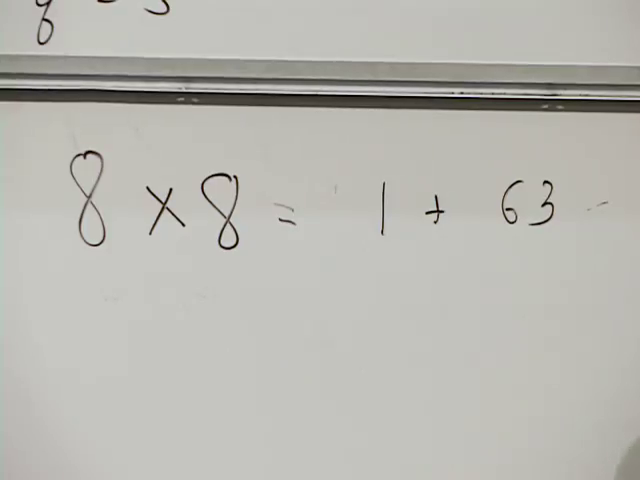
\includegraphics[width=0.68\textwidth]{lecture_04_figure_05.png}\caption{Die Zustandszählung an der Tafel für zwei Gluonen: ein Singulett unter vierundsechzig Zuständen.}\lectureframe{00:53:44}\end{figure}

Die vollständige Zerlegung in irreduzible Darstellungen lautet
\begin{equation}
\boldsymbol 8\otimes\boldsymbol 8
=\boldsymbol 1\oplus\boldsymbol 8_S\oplus\boldsymbol 8_A
\oplus\boldsymbol{10}\oplus\overline{\boldsymbol{10}}
\oplus\boldsymbol{27}.
\label{eq:l4-eight-times-eight}
\end{equation}
Die Dimensionen ergeben zusammen die richtige Gesamtzahl:
\begin{equation}
1+8+8+10+10+27=64.
\end{equation}
Die beiden Oktette sind verschiedene invariante Unterräume: Eines ist unter dem Austausch der beiden adjungierten Faktoren symmetrisch, das andere antisymmetrisch. Das Singulett ist der Farbkanal aus zwei Gluonen, aus dem ein Glueball-Zustand gebildet werden kann.
\editorialnote{An der Tafel steht zunächst nur \(8\times8=1+63\). Der spätere Austausch im Hörsaal ergänzt die angegebenen irreduziblen Dimensionen; Balken und Symmetrieindizes sind hier in der üblichen \(SU(3)\)-Notation wiedergegeben.}

\subsection{Warum beobachtbare elektrische Ladungen ganzzahlig sind}

Die Quarkladungen fallen in zwei Typen:
\begin{equation}
Q_{\mathrm{up\text{-}like}}=+\frac23,
\qquad
Q_{\mathrm{down\text{-}like}}=-\frac13.
\end{equation}
Drei Quarks haben daher eine ganzzahlige Gesamtladung: \(-1,0,+1,\text{ or }+2\), je nachdem, wie viele davon up-artig sind. Ein Quark und ein Antiquark haben ebenso eine Ladung von \(0\) oder \(\pm1\). Gluonen tragen keine elektrische Ladung. Somit haben die grundlegenden Farbsinguletts, die sich aus den beobachteten Quarkdarstellungen bilden, ganzzahlige elektrische Ladung, obwohl ihre Bestandteile gebrochene Ladungen tragen.

\begin{classroomqa}
\audiencequestion{Welche elektrische Ladung hat das Strange-Quark?
\lecturetimestamp{00:56:08}}
\lecturerresponse{Es ist down-artig und hat daher die Ladung \(-1/3\). Die drei Familien wiederholen dasselbe Ladungsmuster: \((u,d)\), \((c,s)\) und \((t,b)\); jedes Paar hat die Ladungen \(+2/3\) und \(-1/3\).}
\end{classroomqa}

Für diesen Teilcheninhalt hängen Farbsingulett-Eigenschaft und ganzzahlige elektrische Ladung eng zusammen, sind aber mathematisch nicht dasselbe. Die Ganzzahligkeit folgt auch aus den gerade angegebenen elektrischen Ladungszuordnungen des Standardmodells.

\begin{classroomqa}
\audiencequestion{Ist ein Farbsingulett ein verschränkter Zustand, und hat diese Verschränkung dieselbe Bedeutung wie die eines verschränkten Paares in einem Bell-Experiment?
\lecturetimestamp{00:56:58}}
\lecturerresponse{Die Farbsingulett-Wellenfunktion ist tatsächlich verschränkt: Sie ist eine kohärente Überlagerung und kein Produkt von Zuständen mit jeweils bestimmter Farbe. Grundsätzlich lassen sich ihre Bestandteile voneinander trennen, doch aufgrund des Confinements wird diese Trennung zunehmend aufwendiger und führt schließlich zur Bildung neuer Hadronen. Daher eignet sich der Zustand nicht für eine Manipulation nach Art eines Bell-Experiments, obwohl er verschränkt ist.}
\end{classroomqa}

\section{Was die Tensorprodukt-Gleichungen bedeuten}

An dieser Stelle verdienen die Multiplikationstafeln eine anschaulichere Erklärung. Seien \(\psi_i\) und \(\phi_j\) Operatoren, die zwei Spin-ein-Halb-Objekte erzeugen. Sie können zwei Teilchensorten wie ein Elektron und ein Proton beschreiben oder, unter Berücksichtigung der passenden Statistik, zwei Exemplare derselben Sorte. Jeder Index kann zwei Werte annehmen. Die vier Produkte
\begin{equation}
\psi_\uparrow\phi_\uparrow,
\quad
\psi_\uparrow\phi_\downarrow,
\quad
\psi_\downarrow\phi_\uparrow,
\quad
\psi_\downarrow\phi_\downarrow
\end{equation}
spannen den Tensorproduktraum auf.

Wirkt ein Gruppenelement auf jeden Faktor wie \(U\), so wirkt es auf das Produkt wie \(U\otimes U\). In Komponenten gilt
\begin{equation}
\psi_i\phi_j
\longmapsto
U_i{}^kU_j{}^\ell\psi_k\phi_\ell.
\label{eq:l4-product-action}
\end{equation}
Dies ist eine vierdimensionale, aber reduzible Darstellung. Die antisymmetrische Kombination
\begin{equation}
\frac{1}{\sqrt2}
(\psi_\uparrow\phi_\downarrow
-\psi_\downarrow\phi_\uparrow)
\end{equation}
wird in sich selbst abgebildet, während die drei symmetrischen Kombinationen untereinander abgebildet werden. In einer an diese Kombinationen angepassten Basis hat jede Matrix der Produktdarstellung Blockdiagonalform:
\begin{equation}
D_{2\otimes2}(g)
\sim
\begin{pmatrix}
1&0\\
0&D_3(g)
\end{pmatrix}.
\label{eq:l4-spin-block-diagonal}
\end{equation}

\begin{classroomqa}
\audiencequestion{Welche Operation stellt eine Gleichung wie \(\boldsymbol 3\otimes\boldsymbol 3=\bar{\boldsymbol 3}\oplus\boldsymbol 6\) dar?
\lecturetimestamp{00:57:51}}
\lecturerresponse{Die linke Seite bildet den zusammengesetzten Zustandsraum. Die Gruppe wirkt auf beide Faktoren und mischt daher die Produktbasiszustände. Die rechte Seite besagt, dass eine Basisänderung diese Zustände in invariante Mengen aufteilt: drei antisymmetrische Kombinationen, die wie ein Antitriplett transformieren, und sechs symmetrische Kombinationen, die wie ein Sextett transformieren. Das Pluszeichen bezeichnet eine direkte Summe von Möglichkeiten, keine gewöhnliche numerische Addition.}
\end{classroomqa}

\begin{classroomqa}
\audiencequestion{Woher wissen wir, dass sich die neun Zustände als \(3+6\) oder als \(1+8\) zerlegen und nicht etwa als \(2+7\)?
\lecturetimestamp{01:04:39}}
\lecturerresponse{Die Dimensionszählung allein entscheidet nicht über die Zerlegung. Man muss wissen, welche irreduziblen Darstellungen \(SU(3)\) besitzt, und invariante Unterräume konstruieren, etwa indem man Indizes symmetrisiert oder antisymmetrisiert oder Spur und spurfreie Anteile trennt. Eine vollständige Klassifikation erfordert mehr Gruppentheorie; hier verwenden wir nur die für Quarks und Gluonen benötigten Darstellungen.}
\end{classroomqa}

Der invariante Epsilon-Tensor macht die Konstruktion des Singuletts anschaulich. Für \(SU(2)\) gilt
\begin{equation}
\epsilon_{ij}U^i{}_kU^j{}_\ell
=(\det U)\epsilon_{k\ell}
=\epsilon_{k\ell}.
\end{equation}
Daher ist \(\epsilon_{ij}\psi^i\phi^j\) invariant. Für \(SU(3)\) ergibt die Variante mit drei Indizes
\begin{equation}
\epsilon_{ijk}U^i{}_aU^j{}_bU^k{}_c
=(\det U)\epsilon_{abc}
=\epsilon_{abc},
\end{equation}
und beweist damit die Invarianz des Drei-Quark-Zustands in Gleichung~\eqref{eq:l4-baryon-singlet}.

\begin{classroomqa}
\audiencequestion{Kann man ausdrücklich zeigen, warum das Singulett nicht transformiert?
\lecturetimestamp{01:07:18}}
\lecturerresponse{Ja. Kontrahiere alle fundamentalen Indizes mit dem vollständig antisymmetrischen Epsilon-Tensor. Bei der Transformation multipliziert das Produkt der Matrizen Epsilon mit \(\det U\). Für eine spezielle unitäre Matrix ist diese Determinante eins, sodass der kontrahierte Zustand unverändert bleibt. Für \(SU(2)\) beweist dies die Zwei-Spin-Singulett-Eigenschaft; für \(SU(3)\) die des Drei-Quark-Singuletts Rot--Grün--Blau.}
\end{classroomqa}

\begin{classroomqa}
\audiencequestion{Wie lautet die vollständige Zerlegung zweier Gluonen-Oktette?
\lecturetimestamp{01:09:24}}
\lecturerresponse{Sie ist die Zerlegung aus Gleichung~\eqref{eq:l4-eight-times-eight}: ein Singulett, zwei Oktette, ein Dekuplett, ein Antidekuplett und eine Darstellung der Dimension siebenundzwanzig. Es gibt genau eine farbsinguläre Kombination der beiden Oktett-Indizes.}
\end{classroomqa}

\begin{classroomqa}
\audiencequestion{Wie lautet die entsprechende vollständige Zerlegung für drei Quarks?
\lecturetimestamp{01:11:51}}
\lecturerresponse{Die physikalisch wesentliche Antwort ist, dass sie ein Singulett enthält. Ergänzt man die vollständige Zerlegung, erhält man Gleichung~\eqref{eq:l4-three-quark-full}: ein Singulett, zwei Oktette und ein Dekuplett, insgesamt also \(1+8+8+10=27\) Zustände.\editorialnote{Während des Austauschs kann sich der Dozent nicht an die vollständige Zerlegung \(3\otimes3\otimes3\) erinnern. Die übliche Ergänzung wird hier ausdrücklich angegeben und nicht der gesprochenen Antwort zugeschrieben.}}
\end{classroomqa}

Dieselbe Idee lässt sich auf den Zweigluonenraum übertragen. In der naiven Produktbasis wirkt \(SU(3)\) durch \(64\times64\)-Matrizen. In einer an die irreduziblen Komponenten angepassten Basis sind diese Matrizen blockdiagonal,
\begin{equation}
\begin{aligned}
D_{8\otimes8}(g)
&\sim
\operatorname{diag}\bigl(
1,D_{8_S}(g),D_{8_A}(g),
\\
&\hspace{4.8em}
D_{10}(g),D_{\overline{10}}(g),D_{27}(g)
\bigr).
\end{aligned}
\end{equation}
Kein Block mischt sich mit einem anderen, obwohl sich die Zustände innerhalb jedes Blocks untereinander mischen.

\begin{classroomqa}
\audiencequestion{Ist die Zerlegung des Tensorprodukts also einfach ein Basiswechsel, bei dem die große Darstellungsmatrix blockdiagonal wird?
\lecturetimestamp{01:12:02}}
\lecturerresponse{Genau. Bei zwei Spins zerfällt die vierdimensionale Matrix in einen eindimensionalen Singulettblock und einen dreidimensionalen Triplettblock. Bei zwei Gluonen zerfällt die 64-dimensionale Matrix in Blöcke der Dimensionen \(1,8,8,10,10,\text{ and }27\). Jeder Block ist unter jeder Gruppentransformation abgeschlossen.}
\end{classroomqa}

\begin{classroomqa}
\audiencequestion{Gibt es eine Bezeichnung für eines dieser abgeschlossenen Teilstücke im gesamten Tensorproduktraum?
\lecturetimestamp{01:14:55}}
\lecturerresponse{Es ist ein invarianter Unterraum, der eine Unterdarstellung trägt. Lässt es sich nicht weiter zerlegen, trägt es eine irreduzible Darstellung, kurz Irrep. Das gesamte Tensorprodukt ist die direkte Summe dieser irreduziblen Komponenten.\editorialnote{Im Ausgangstext bleibt der gesuchte Begriff im Hörsaal unbeantwortet. Die Antwort ergänzt den gebräuchlichen Begriff aus der Darstellungstheorie.}}
\end{classroomqa}

\begin{classroomqa}
\audiencequestion{Wenn die Nichtsingulett-Dekupletts und andere Darstellungen als nicht existent bezeichnet werden, heißt das, dass man sie vollständig ignorieren sollte?
\lecturetimestamp{01:15:36}}
\lecturerresponse{Sie sind zulässige Farbsektoren und spielen in Zwischenrechnungen eine Rolle, treten im Labor aber nicht als isolierte Teilchen endlicher Energie auf. Nicht ein Versagen der Darstellungstheorie, sondern das Confinement verhindert, dass sie zu freien asymptotischen Zuständen werden.}
\end{classroomqa}

\section{Von Nambus Farbidee zum Confinement}

Die Farbidee entstand vor der endgültigen Formulierung der QCD. Yoichiro Nambu erkannte bereits in den frühen 1960er Jahren, dass eine verborgene dreifachwertige Quantenzahl ein verblüffendes Problem lösen könnte: Quarks tragen eine gebrochene elektrische Ladung, doch freie Teilchen mit gebrochener Ladung werden nicht beobachtet. Wenn physikalische Zustände auf Farbsinguletts beschränkt sind, treten Quarks in den oben beschriebenen Kombinationen mit ganzzahliger Ladung auf. Die verbleibende Frage ist dynamischer Natur: Welche Kräfte zwingen alle freien Zustände endlicher Energie, Singuletts zu sein?

Beginnen wir mit der Analogie zur Elektromagnetismus. Eine Ladung und eine entgegengesetzte Ladung ziehen sich an. Bringt man sie zusammen, sinkt die Energie; gleichnamige Ladungen zusammenzuschieben erfordert Arbeit. Das Feld selbst speichert positive Energie,
\begin{equation}
E_{\mathrm{field}}
=\frac12\int d^3x\,\boldsymbol E^2
\end{equation}
in einfachen elektrostatischen Einheiten. Bei einer Nettoladung reicht das Feld weit über das System hinaus, während ein eng gebundenes neutrales Paar nur ein Dipolfeld kurzer Reichweite besitzt. Durch die Neutralisierung wird daher Feldenergie aus dem Außenraum entfernt.

Stellen wir uns vor, die elektromagnetische Kopplung würde enorm vergrößert. Die Feldenergiekosten einer Nettoladung würden so hoch, dass Objekte niedriger Energie überwiegend neutral wären und das Herauslösen eines geladenen Bestandteils unerschwinglich teuer werden könnte. Nambu übertrug diese Vorstellung auf die Farbe: Die acht Farbladungen sind Quellen von acht Gluonenfeldern, sodass eine große Farbfeldenergie isolierte Nichtsinguletts ausschließen könnte.

Diese Vorstellung trifft im Wesentlichen zu, doch die QCD weist ein entscheidendes neues Merkmal auf. Das Photon trägt keine elektrische Ladung, das Gluon hingegen Farbe. Das Photon ist keine Quelle des klassischen elektromagnetischen Feldes, und die Maxwell-Gleichungen sind linear: Zwei elektromagnetische Wellen überlagern sich und durchdringen einander. Ein Gluon transformiert in der Farboktett-Darstellung, daher sind Gluonen Quellen anderer Gluonen und wechselwirken mit ihnen. Auch verschiedene Teile eines einzelnen Gluonenfeldes wechselwirken miteinander. Das nichtabelsche Eichfeld ist deshalb nichtlinear.

\subsection{Flussschläuche und ein lineares Potenzial}

Auf großen Distanzen verhindert die Selbstwechselwirkung der Gluonen, dass sich der Farbfluss wie das gewöhnliche elektrische Dipolfeld ausbreitet. Der Fluss wird in einen Schlauch eingeschnürt, der ein Quark mit einem Antiquark verbindet. Feldstärke und Querschnittsfläche eines langen Schlauchs sind näherungsweise konstant, sodass der Schlauch näherungsweise eine konstante Energie pro Längeneinheit speichert. Bezeichnet \(\sigma\) die Stringspannung, so gilt
\begin{equation}
V(R)\simeq\sigma R+\text{constant}
\qquad (R\ \text{large}).
\label{eq:l4-linear-potential}
\end{equation}

\begin{figure}[htbp]
\centering
\includegraphics[width=0.78\textwidth]{lecture_04_figure_06.png}
\caption{In einem langen Schlauch gebündelter Farbfluss zwischen einem Quark und einem Antiquark.}
\lectureframe{01:31:35}
\end{figure}

Dies ist stärker als das Coulomb-Potenzial, dessen Betrag wie \(1/R\) abnimmt. Zieht man die Farbquellen weiter auseinander, wird die Kraft nicht immer schwächer; der Schlauch wird länger und seine Energie nimmt weiter zu. Eine einzelne Farbladung in einem unendlichen Volumen würde einen endlos langen Schlauch erfordern und damit unbeschränkte Energie. Das ist die physikalische Bedeutung der Aussage, dass nur Farbsinguletts asymptotische Zustände endlicher Energie sind.
\editorialnote{Die Notation für die Stringspannung und das explizite langreichweitige Potenzial machen die Aussage der Quelle quantitativ, dass ein gleichförmiger Flussschlauch eine gleichförmige Energie pro Längeneinheit trägt.}

\subsection{Stringbruch und Jets}

Nehmen wir an, eine harte Kollision trifft ein Quark in einem Meson. Das Quark beginnt sich fortzubewegen, doch hinter ihm spannt sich der Flussschlauch. Es kann seine kinetische Energie verlieren und zurückgezogen werden. Häufiger erzeugt das Vakuum, sobald die gespeicherte Feldenergie groß genug ist, ein neues Quark--Antiquark-Paar. Das neue Antiquark beendet den Fluss, der mit dem entkommenden Quark verbunden ist, während das neue Quark den Fluss zum ursprünglichen Antiquark beendet. Aus einem gedehnten Singulett werden zwei kürzere Singuletts,
\begin{equation}
(q\bar q)_{\mathrm{stretched}}
\longrightarrow
(q\bar q)+(q\bar q).
\label{eq:l4-string-breaking}
\end{equation}

\begin{figure}[htbp]
\centering
\includegraphics[width=0.78\textwidth]{lecture_04_figure_07.png}
\caption{Paarerzeugung bricht einen gedehnten Flussschlauch in zwei farbsingulettartige Schläuche auf.}
\lectureframe{01:34:52}
\end{figure}

\begin{classroomqa}
\audiencequestion{Was kann noch geschehen, wenn ein getroffenes Quark genug Energie hat, um den Schlauch weiter zu dehnen, außer dass es zurückgezogen wird?
\lecturetimestamp{01:33:50}}
\lecturerresponse{Der Schlauch kann durch die Erzeugung eines Quark--Antiquark-Paares aufbrechen. Seine Energie wird zur Masse und kinetischen Energie des neuen Paares. Die Endpunkte verbinden sich neu zu zwei Singuletts, sodass der Prozess zusätzliche Mesonen statt eines isolierten Quarks erzeugt.}
\end{classroomqa}

Wenn eines dieser Partonen weiterhin großen Impuls trägt, wiederholt sich der Prozess. Das Ergebnis ist eine Kaskade von farbsingulettartigen Hadronen, die um die ursprüngliche Partonrichtung gebündelt sind: ein Jet. Diese Umwandlung energiereicher Quarks und Gluonen in Hadronen heißt Hadronisierung. Auf das initiierende farbgeladene Objekt schließt man aus dem Jet, beobachtet wird es niemals für sich allein.

\begin{classroomqa}
\audiencequestion{Entstehen beim Stringbruch nur Mesonen, oder können im Jet auch andere Hadronen auftreten?
\lecturetimestamp{01:35:20}}
\lecturerresponse{Gewiss können auch andere Hadronen auftreten. Die einzige Farbanforderung ist, dass die letztlich beobachtbaren Objekte Singuletts sind. Mesonen sind das einfachste Bild für einen einzelnen Bruch, doch es können auch Baryonen, Antibaryonen und kompliziertere Singulettkombinationen entstehen.}
\end{classroomqa}

Drei Quarks können ihren Fluss an einem farbsingulettartigen Knotenpunkt beenden. Das Bild mit den drei Strängen ist das dynamische Gegenstück zum antisymmetrischen Epsilon-Tensor in Gleichung~\eqref{eq:l4-baryon-singlet}: Aus dem vollständigen Baryon tritt kein Nettofarbfluss aus.

\begin{figure}[htbp]
\centering
\includegraphics[width=0.72\textwidth]{lecture_04_figure_08.png}
\caption{Ein dreisträngiger Farbfluss-Knotenpunkt für ein Baryon, unterhalb der Skizze zum Stringbruch bei Mesonen.}
\lectureframe{01:36:12}
\end{figure}

\section{Eichfelder, Erhaltungsgrößen und das Standardmodell}

Auf der hier betrachteten Ebene lässt sich eine Eichtheorie als Theorie erkennen, in der eine erhaltene Ladung eine photonartige Feldquelle ist. Die elektrische Ladung ist Quelle des elektromagnetischen Feldes; die acht Farbladungen sind Quellen der acht Gluonenfelder. In der tiefer gehenden Formulierung wird die Symmetrie lokal gemacht und eine Verbindung eingeführt, die innere Zustände an benachbarten Raumzeitpunkten vergleicht. Diese Konstruktion wird für das hier entwickelte Bild des Confinements jedoch nicht benötigt.
\editorialnote{Die Formulierung mit lokaler Symmetrie ist die gebräuchliche tiefer gehende Bedeutung von Eichtheorie, auf die die Quelle anspielt, deren Erörterung sie aber bewusst aufschiebt.}

Symmetrie, erhaltene Ladung und Fluss hängen eng zusammen. Können Feldlinien nur an Ladungen enden, kann eine Quelle nicht einfach verschwinden, während ihr Fluss an nichts mehr gebunden ist. Auch kann ihr entferntes Feld nicht augenblicklich vollständig verschwinden, denn Änderungen des Feldes breiten sich kausal aus. In lokaler Form wird dieselbe Physik durch eine Kontinuitätsgleichung ausgedrückt,
\begin{equation}
\frac{\partial\rho}{\partial t}
+\boldsymbol\nabla\cdot\boldsymbol j=0,
\end{equation}
die besagt, dass Ladung ein Gebiet nur verlassen kann, indem sie dessen Grenze durchströmt. Das Bild der Feldlinien ist die geometrische Darstellung dieses lokalen Erhaltungsgesetzes.

Nun können wir das Ergebnis im Standardmodell verorten. Die Farbe umfasst die acht Generatoren von \(SU(3)\) und ihre acht Gluonenfelder. Der abelsche Sektor enthält einen Generator und ein Eichfeld. Drei weitere Generatoren gehören zu einer zusätzlichen \(SU(2)\), nicht zum gewöhnlichen räumlichen Drehimpuls. Vor der Symmetriebrechung lautet die Eichstruktur
\begin{equation}
SU(3)_c\times SU(2)_L\times U(1)_Y,
\end{equation}
mit \(8+3+1=12\) Generatoren. Als Nächstes gilt es, die elektroschwache \(SU(2)\) zu verstehen, dann das Higgs-Feld und die Entstehung des beobachteten Photons, von \(W^\pm\) und \(Z\).
\editorialnote{Die Quelle zählt das Photon zusammen mit den acht Gluonen und beschreibt den verbleibenden Faktor als \(SU(2)\times U(1)\). Im ungebrochenen Standardmodell ist der abelsche Faktor die Hyperladung \(U(1)_Y\); das Photon entsteht erst durch die elektroschwache Mischung.}

Die zentrale Argumentationskette ist nun vollständig. Abstrakte Gruppen wirken durch Darstellungen; infinitesimale Generatoren sind die erhaltenen Ladungen; Quarks, Antiquarks und Gluonen gehören zur \(\boldsymbol 3\)-, \(\bar{\boldsymbol 3}\)- beziehungsweise \(\boldsymbol 8\)-Darstellung; Tensorprodukte identifizieren die singulettartigen Hadronen; und das nichtlineare Gluonenfeld macht aus der Singulettauswahl das physikalische Phänomen des Confinements.
